%!TEX encoding = UTF-8 Unicode
\documentclass[
    fontsize=12pt,
    headings=small,
    parskip=half,           % Ersetzt manuelles setzten von parskip/parindent.
    bibliography=totoc,
    numbers=noenddot,       % Entfernt den letzten Punkt der Kapitelnummern.
    open=any,               % Kapitel kann auf jeder Seite beginnen.
%   final                   % Entfernt alle todonotes und den Entwurfstempel.
    ]{scrreprt}

% ===================================Praeambel==================================

% Kodierung, Sprache, Patches {{{
\usepackage[T1]{fontenc}    % Ausgabekodierung; ermoeglicht Akzente und Umlaute
                            %  sowie korrekte Silbentrennung.
\usepackage[utf8]{inputenc} % Erlaub die direkte Eingabe spezieller Zeichen.
                            %  Utf8 muss die Eingabekodierung des Editors sein.
\usepackage[ngerman]{babel} % Deutsche Sprachanpassungen (z.B. Ueberschriften).
\usepackage{microtype}      % Optimale Randausrichtung und Skalierung.
\usepackage[
    autostyle,
    ]{csquotes}             % Korrekte Anfuehrungszeichen in der Literaturliste.
\usepackage{fixltx2e}       % Patches fuer LaTeX2e.
\usepackage{scrhack}        % Verhindert Warnungen mit aelteren Paketen.
% }}}

% Schriftarten {{{
\usepackage{mathptmx}       % Times. Package 'times.sty' is obsolete.
\usepackage[scaled=.92]{helvet}
\usepackage{courier}
% }}}

% Dokument- und Texteinstellungen {{{
\usepackage[
    a4paper,
    margin=2.54cm,
    marginparwidth=2.0cm,
    footskip=1.0cm
    ]{geometry}             % Ersetzt 'a4wide'.
\clubpenalty=10000          % Keine Einzelzeile am Beginn eines Paragraphen
                            %  (Schusterjungen).
\widowpenalty=10000         % Keine Einzelzeile am Ende eines Paragraphen
\displaywidowpenalty=10000  %  (Hurenkinder).
\usepackage{floatrow}       % Zentriert alle Floats.
\usepackage{ifdraft}        % Ermoeglicht \ifoptionfinal{true}{false}
\pagestyle{plain}           % keine Kopfzeilen
% \sloppy                     % großzügige Formatierungsweise
\deffootnote{1em}{1em}{\thefootnotemark.\ } % Verbessert Layout mehrzeiliger Fußnoten

\makeatletter
\AtBeginDocument{%
    \hypersetup{%
        pdftitle = {\@title},
        pdfauthor  = \@author,
    }
}
\makeatother
% }}}

% Weitere Pakete {{{
\usepackage{graphicx}       % Einfuegen von Graphiken.
\usepackage{tabu}           % Einfuegen von Tabellen.
\usepackage{multirow}       % Tabellenzeilen zusammenfassen.
\usepackage{multicol}       % Tabellenspalten zusammenfassen.
\usepackage{booktabs}       % Schönere Tabellen (\toprule\midrule\bottomrule).
\usepackage[nocut]{thmbox}  % Theorembox bspw. fuer Angreifermodell.
\usepackage{amsmath}        % Erweiterte Handhabung mathematischer Formeln.
\usepackage{amssymb}        % Erweiterte mathematische Symbole.
\usepackage{rotating}
\usepackage[
    printonlyused
    ]{acronym}              % Abkuerzungsverzeichnis.
\usepackage[
    colorinlistoftodos,
    textsize=tiny,          % Notizen und TODOs - mit der todonotes.sty von
    \ifoptionfinal{disable}{}%  Benjamin Kellermann ist das Package "changebar"
    ]{todonotes}            %  bereits integriert.
\usepackage[
    breaklinks,
    hidelinks,
    pdfdisplaydoctitle,
    pdfpagemode = {UseOutlines},
    pdfpagelabels,
    ]{hyperref}             % Sprungmarken im PDF. Laed das URL Paket.
    \urlstyle{rm}           % Entfernt die Formattierung von URLs.
\usepackage{breakurl}
\def\UrlBreaks{\do\/\do-}
\usepackage{listings}       % Spezielle Umgebung für...
    \lstset{                %  ...Quelltextformatierung.
        language=C,
        breaklines=true,
        breakatwhitespace=true,
        frame=L,
        captionpos=b,
        xleftmargin=6ex,
        tabsize=4,
        numbers=left,
        numberstyle=\ttfamily\footnotesize,
        basicstyle=\ttfamily\footnotesize,
        keywordstyle=\bfseries\color{green!50!black},
        commentstyle=\itshape\color{magenta!90!black},
        identifierstyle=\ttfamily,
        stringstyle=\color{orange!90!black},
        showstringspaces=false,
        }
% }}}

% ===================================Dokument===================================

\title{Das cMix-Verfahren}
\author{todo}
% \date{01.01.2015} % falls ein bestimmter Tag eingesetzt werden soll, einfach diese Zeile aktivieren

\begin{document}

\begin{titlepage}
\begin{center}\Large
    Universität Hamburg \par
    Fachbereich Informatik
    \vfill
    \makeatletter
    {\Large\textsf{\textbf{\@title}}\par}
    \makeatother
    \bigskip
    am Arbeitsbereich Sicherheit in Verteilten Systemen (SVS) \par
    \bigskip
    \makeatletter
    {\@author} \par
    \makeatother
    \bigskip
    \makeatletter
    {\@date}
    \makeatother
    \vfill

\end{center}
\end{titlepage}

\tableofcontents

\chapter{Abstract / Einleitung}
\textit{Das ist die Zusammenfassung}

In der heutigen Zeit sind Nachrichten, welche über das Internet versendet werden, nicht
mehr weg zu denken. Zunehmend fragen sich die Benutzer ob ihre Anonymität bei
Benutzung von Mails und Messengern gewährleistet wird. Deshalb gibt es in der IT-Sicherheit Verfahren, die die Anonymität des Nutzers sicherstellen. Das C-Mix Verfahren, mit welchem wir uns in der
vorliegenden Ausarbeitung auseinandersetzen, ist ein solches Verfahren. Es
wurde von David Chaum konzipiert und ist eine
Weiterentwicklung, der ebenso von ihm entwickelten Chaumschen Mixe aus dem Jahr
1981. Da die Chaumschen Mixe und Nachfolger nicht effizient sind,
wurde das C-Mix Verfahren entwickelt.
Wir wollen uns in dieser Ausarbeitung
näher damit beschäftigen, ob das Problem mit dem C-Mix verfahren gelöst wurden ist
und ob das Verfahren neue Probleme bereit hält.
Die Ausarbeitung orientiert sich am Paper \cite{DBLP:journals/iacr/DavidChaumJKKRS16} von David Chaum et al.


\chapter{Übersicht Chaumsche Mixe}

\section{Funktionsprinzip}

Die Chaumsche Mixe gewährleisten die Anonymität der
Kommunikation, indem sie Sender und Empfänger voreinander anonym halten. 
Dies
gelingt, indem die zu verschickenden Nachrichten mehrere Stationen - sogenannte
Mixe - durchlaufen. Diese sorgen dafür, dass die Nachrichten, sowohl Empfänger als
auch Sender nicht zueinander in Beziehung gesetzt werden können.

Zum einen muss ein Mix die Nachrichten mithilfe eines Verschlüsselungssystems verschlüsseln und ein anderer
später wieder entschlüsseln. 

Durch diese Methode des Umkodieren ist es nicht mehr
möglich eine Beziehung zwischen Eingangs und Ausgangsnachrichten zu finden. 

Ein anderer Mix muss die Nachrichten sammeln und ein weiterer umsortieren, damit
man nicht ausgehend von der Reihenfolge des Eintreffens und Weiterleitens der
Nachrichten am Mix eine Beziehung zwischen Sender und Empfänger vorfinden
kann. 

Mithilfe einer Rückadresse, die als Teil einer Nachricht gesendet wird und
einem Mix, der diese Rückadresse zwischen speichert und umkodiert, können sich
zwei Nutzer nun gegenseitig Nachrichten senden und dabei anonym bleiben.  \cite{Chaum:1981:UEM:358549.358563} \cite{sampigethaya2006survey}

\section{Probleme}

Die Chaumsche Mixe haben durchaus ihre Grenzen, innerhalb eines Echtzeitsystems
ist das Sammeln der Nachrichten sehr ineffizient, da man durchaus lange warten
muss um mehrere Nachrichten zusammen zu bekommen. Deshalb wird in solchen
Echtzeitsystemen das Sammeln der Nachrichten weggelassen oder kurz gehalten.
Das Umsortieren der Nachrichten kann deshalb nicht oder nur mit wenig Nachrichten
erfolgen. Daraus resultiert, dass die Sicherheit sinkt und das ganze Verfahren in
Echtzeitsystemen somit angreifbarer wird. \cite{Chaum:1981:UEM:358549.358563} \cite{sampigethaya2006survey}

\chapter{Das cMix Verfahren}

\section{Idee}

Die grundsätzliche Idee des cMix Verfahrens ist es, Schlüsselberechnungen in Echzeit zu vermeiden. Hierdurch entsteht auf 
der einen Seite eine Steigerung der Effizienz von Mix-Netzen, d.h. bessere Performance, also weniger verzögerte Kommunikation. Auf der anderen Seite wird
 der Energiebedarf verringert, was z.B. zu längerer Akkulaufzeit eines Smartphones führen kann.
 Um dies zu erreichen werden vor der eigentlichen Kommunikation Schüssel berechechnet (Precomputation) und zwischen dem Sender und den Mix-Nodes ausgetauscht.
 Diese werden dann als Seed für einen Pseudozufallsgenerator verwendet, um weitere (gleiche) Schlüssel zu erzeugen.
 
Folgendes Funktionprinzip und die Analyse stammt aus \cite{DBLP:journals/iacr/DavidChaumJKKRS16}.


\section{Funktionsprinzip}
\subsection{Übersicht}
Seien $m$ die Anzahl der Nutzer des cMix-Systems mit $n$ Mixknoten $N_1, N_2, ... ,  N_n$. 

Sei $T$ ein Netzwerkknoten, welcher eingehende Nachrichten in Bündeln sortiert und zur weiteren Kommunikation dient.

$\beta$ Anzahl der Nachrichten, die ein Knoten gleichzeitig verarbeiten kann, wobei $\beta \geq m$ gilt.

\begin{figure}[h]
 \caption{Übersicht der Kommunikation}
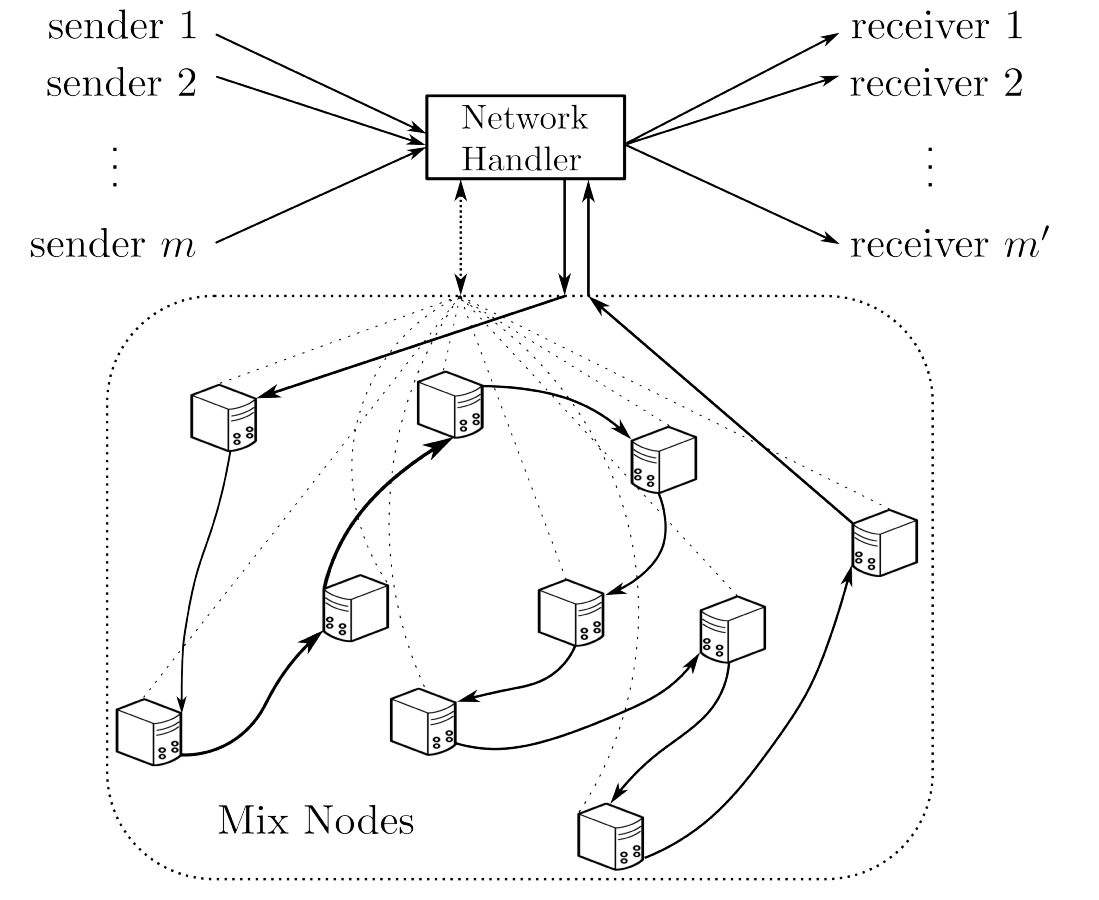
\includegraphics[width=0.5\textwidth]{Bilder/commu_model.png} \label{graphic:commu}
\end{figure}



\subsection{Pre-Communication}

Vor der Benutzung des System, muss jeder Nachrichtensender jeweils einen symmetrischen Schlüssel mit jedem der Mixknoten austauschen.
Für jeden Knoten $N_i$ und jeden Nutzer $U_j$ sei dieser Schlüssel $MK_{i,j}$.
Dieser Schlüssel wird z.B. mit Hilfe des Diffie-Hellman Verfahrens ausgetauscht.

Bei Kommunikation mit dem Mixnetz, ver- oder entschüsselt jeder Teilnehmer jede seiner Nachrichten mit Schlüsseln, die aus den gemeinsamen Schlüsseln \(MK_{i,j}\) erzeugt werden.
Genauer gesagt, werden diese Schlüssel als Ausgabe eines Pseudozufallszahlengeneratoren berechnet, welche bei gleichem Startwert die gleiche Zahlenfolge generieren.
Als Startwert werden hier die Schüsselpaare \(MK_{i,j}\) verwendet, so dass Nutzer und Mixknoten jeweils die gleichen Keys erzeugen.
Die pseudozufallsgenerierten Schlüssel sind als \(ka_{i,j}\) bezeichnet.
Zum Verschlüsseln einer Nachricht, berechnet der Nutzer aus den Schlüsseln \(MK_{i,j}\)
einen zusammengesetzten Schüssel: \(Ka_j = \prod_{i=1}^{n} ka_{i,j}\),
dann kann die Nachricht \(M_1\) durch \(M_1 \times Ka_{j}^{-1}\) verschlüsselt werden.

Außerdem legt jeder Mixknoten eine zufällige Permutation $P_i$ fest, die später zum Mixen verwendet wird.

cMix verabeitet jedes Bündel von Nachrichten in zwei Phasen:
\begin{itemize}
	\item Vorberechungsphase (precomputation)
	\item Echzeitphase (real-time)
\end{itemize}

Für den Hinweg von Nachrichten gibt es drei Phasen,
für den Rückweg - also eine Antwort - zwei Phasen.


\subsection{Precomputation Phase}

In der Vorberechnungsphase werden die Werte und Schlüssel berechnet, die später für die Echtzeitphase benötigt werden.
\subsubsection{Vorwärts}
\begin{enumerate}
	\item  \textit{Preprocessing} \\
	Für die Precomputation wird als erster Schritt von jedem Mixknoten $N_i$ eine zufälliger Wert $r_{i,j}$ für jede spätere Nachricht $M_j$ generiert.
Jeder Mixknoten verschlüsselt mittels Elgamal-Verschlüsselungsverfahren
das Inverse des jeweiligen Wertes, also \(r_{i,j}^{-1}\) und sendet das Resultat \(\mathcal{E} (r_i^{-1})\) an den Netzwerknoten $T$.
Der Netzwerknoten $T$ berechnet das komponentenweise direkte Produkt \(\mathcal{E}( R_n^{-1})=\prod_{i=1}^n \mathcal{E} (r_i^{-1})\) der verschlüsselten Vektoren \(\mathcal{E} (r_i^{-1})\) und sendet das Resultat an den ersten Mixknoten.
	
	\item \textit{Mixing} \\
	Im zweiten Schritt der Precomputation permutiert jeder Mixknoten $N_i$ nacheinander das direkte Produkt mit der Anfangs festgelegten Permutation $P_i$, es wird ein weiterer Vektor \(S_i^{-1} \) mit zufälligen Werten hinzumultipliziert und alles an den nächsten Mixknoten gesendet.
Der letzte Mixknoten hat also den Output \(\mathcal{E} ((P_n(R_n) \times S_n )^{-1})\),
wobei $P_n$ aus den Kompisitionen aller $P_i$'s besteht und $S_n$ das direkte Produkt der $S_i$'s darstellt.
Dieser Output wird wiederum an den Netzwerkknoten gesendet.

	\item \textit{Postprocessing} \\
	Dann wird im dritten Schritt der Precomputation von jedem Mixknoten $N_i$ 
der Entschüsselungsteil $D(i,x)$ aus \(\mathcal{E} ((P_n(R_n) \times S_n )^{-1})\) berechnet.

Hierfür wird eine Methode verwendet, die auf der ElGamal Verschlüsselung basiert,
Eigenschaften von Gruppenhomomorphismen verwendet und hier nicht weiter behandelt wird.
Der interessierte Leser kann in \cite{benaloh2006simple} mehr dazu erfahren.

Um die Entschlüsselung durchzuführen, müsste ein Knoten alle $D(i,x)$ kennen.
\end{enumerate}

\subsubsection{Rückwärts}
\begin{enumerate}
	\item \textit{Mixing} \\
	Der Rückweg funktionier ähnlich wie der Hinweg, allerdings beginnt hier der letzte Mixknoten mit dem Mixing und die Permutationen sind alle umgekehrt, außerdem wird hier kein zufälliger Wert
	$r_{i,j}$ mit einbezogen.
	
	\item \textit{Postprocessing} \\
	Auch für den Rückweg wird wieder ein Entschlüsselungsteil berechnet.
	
\end{enumerate}

\begin{figure}[h]
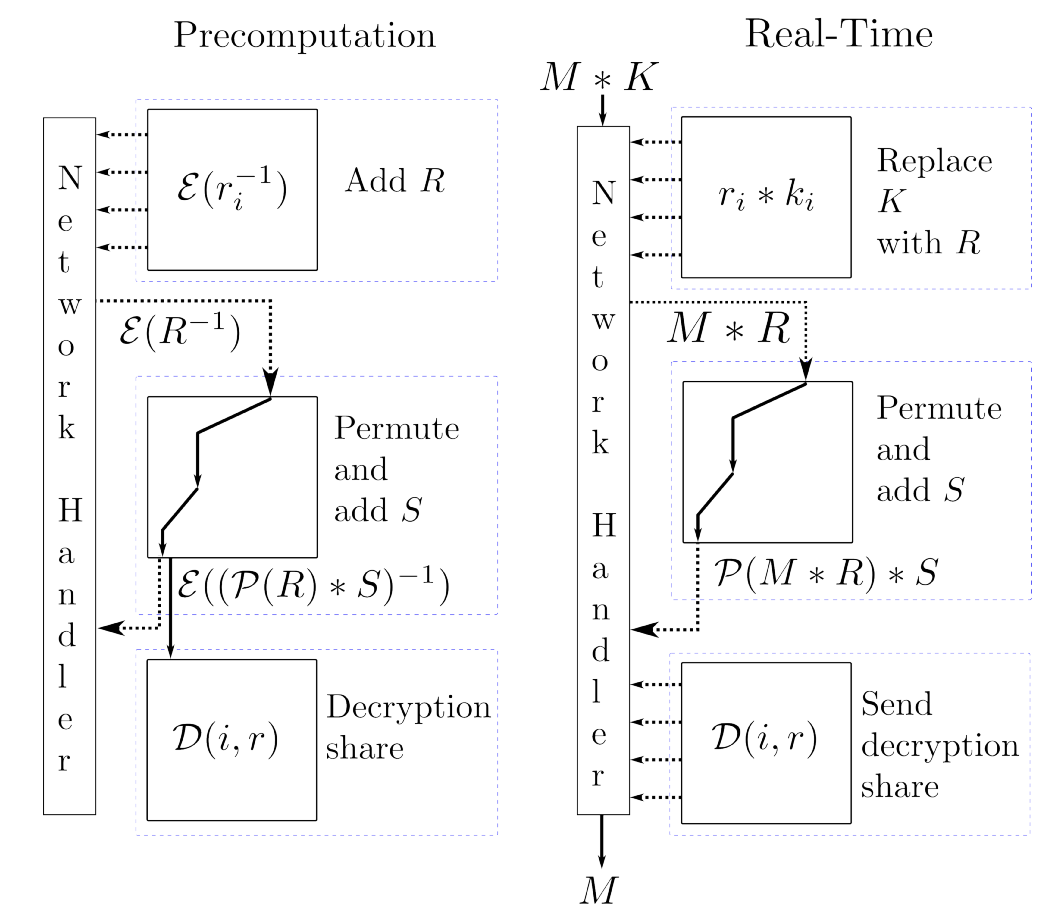
\includegraphics[width=0.8
\textwidth]{Bilder/cmix_overview.png}
 \caption{cMix Overview - Hinweg} \label{graphic:overview}
\end{figure}

\subsection{Echzeit Phase}

In der Echzeitphase generiert nun jeder Nutzer $U_j$ aus dem Schlüssel $MK_{i,j}$
für jeden Mixknoten $M_i$ einen Schlüssel \(ka_{i,j}\) und berechnet dadurch das Produkt:
\(Ka_j = \prod_{i=1}^{n} ka_{i,j}\).\\
Dann sendet jeder Nutzer \(M_j \times Ka_j^{-1}\) an den Netzwerkknoten, welcher diese zu \(M_j \times Ka^{-1}\) kombiniert.

\subsubsection{Vorwärts}
\begin{enumerate}
	\item \textit{Preprocessing} \\
	Als erster Schritt sendet jeder Mixknoten $N_i$ das Produkt aus den gemeinsam genutzen Schlüsseln $ka_i$ und seinen zufällig generierten Werten als Vektor $r_i$ an den Netzwerkknoten.
Dieser multipliziert diese Werte dann mit den Nachrichten von den Sendern.
Damit wird aus $M \times Ka^{-1}$ das Produkt \(M \times R = M_j \times Ka^{-1} \times \prod_{i=1}^{n} ka_{i} \times r_i \).
	
	\item \textit{Mixing} \\
	Im zweiten Schritt der Echzeit-Phase permutiert jeder Mixknoten $N_i$ nacheinander die Nachrichten mit der festgelegten Permutation $p_i$ und multipliziert den in der Vorberechnungsphase - Schritt 2 generierten Vektor $S_i$ von zufälligen Werten $s_i$ hinzu, also ensteht
	\(P_i (M \times R_n) \times S_i\).\\
Das Resultat des letzten Mixknotens ist \(P_n(M \times R_n) \times S_n\).
Dieses wird an den Netzwerkknoten gesendet.

	
	\item \textit{Postprocessing} \\
Im letzten Schritt des Hinwegs, gibt jeder Mixknoten seinen Entschüsselungsanteil $D(i,x)$ an den Netzwerkknoten, welcher dadurch die Nachrichten entschlüsseln, aber nicht mehr mit einem Sender verknüpfen kann.
\begin{eqnarray*}
&P_n (M \times R_n) \times S_n \times \prod_{i=1}^n D(i,x)  \\
=& P_n(M \times R_n) \times S_n \times  (P_n(R_n) \times S_n)^{-1}  \\
=& P_n(M)  \\
\end{eqnarray*}
\end{enumerate}
\subsubsection{Rückwärts}
\begin{enumerate}
	\item \textit{Mixing} \\
	Der Rückweg funktionier ähnlich wie der Hinweg, nur dass der letzte Mixknoten beginnt, die Permutationen alle umgekehrt sind und hier kein zufälliger Wert
	$r_{i,j}$ mit einfließt.
	
	
	\item \textit{Postprocessing} \\
	Für den Rückweg wird der Entschlüsselungsanteil  \(D(i,x)\)
	 in die Schlüssel \(ka_i'\) mit einberechnet, so dass jeder User \(U_J\) aus dem Resultat \(P'_n(M') \times Ka' \) mit seinem Schlüssel \(Ka_j^{'-1}\) seinen Anteil der Nachricht entschlüsseln kann.



\end{enumerate}

\section{Analyse}


\subsection{Sicherheit}

Chaum et al. untersuchen in ihrer Arbeit über cMix auch die Sicherheit des entwickelten Verfahrens.

\subsubsection{Anonymität}

Hierfür wird zuerst eine "ideale Welt" betrachtet, ein Modell, bei der jeder Mixknoten jeweils privat mit den anderen Mixknoten und zusätzlich mit einem vertraulichen dritten Punkt kommunizieren kann.
In diesem Modell gibt es keine kryptografischen Operationen wie Ver- und Entschlüsselung, diese werden hier durch den vertraulichen dritten Punkt sichergestellt.
Dann wird gezeigt, dass dieses Modell die Anonymität des Senders gewährleistet.

Von diesem Modell wird eine \glqq reale Simulation\grqq abstrahiert, wobei Eigenschaften des Modells durch Eigenschaften des cMix Protokolls ersetzt werden.
Damit wird gezeigt, dass cMix das Modell erfüllt und somit Anonymität sicherstellt.

\subsubsection{Integrität}

Die Integrität ist nach Chaum nur gegeben, wenn von den folgenden Bedingungen eine zutrifft.
\begin{itemize}
\item Die Nachricht $M$ wird unmodifiziert an den Empfänger weitergeleitet.
\item Alle Mixknoten wissen, dass das cMix Protokoll nicht richtig durchgeführt wurde.
\end{itemize}

Auf den ersten Punkt wird in diesem Paper nicht weiter eingegangen.
Für den zweiten Punkt wird ein Mechanismus mit dem Namen "Randomized Partial Checking" (vergleiche \cite{jakobsson2002making}) verwendet, welches eine deterministische Verifkation aller ausgehenden Nachrichten im Vergleich zu deren permutierten Eingangsnachrichten durchführt. 
Hierbei wird neben der Integrität auch sichergestellt, dass die Permutationen korrekt ausgeführt werden.

\subsubsection{Vertraulichkeit}

Das cMix Protokoll dient in erster Linie dem Schutzziel \textit{Anonymität},
damit für die zu übermitteldenen Nachrichten auch Vertraulichkeit sichergestellt werden soll, müssen diese vorher vom Sender verschlüsselt werden (z.B. duch einen öffentlichen Schlüssel einer assymetrischen Verschlüsselung).
Es ist aber auch möglich, diese Verschüsselung ohne großen Rechenaufwand in das cMix Verfahren einzubauen, wodurch wiederum aufwändige Publickey-Operationen vermieden werden.

\subsection{Performance}

Die Performance wird durch Chaum et al. auf der einen Seite analysiert, aber auch mit Hilfe eines entwickelten Protoypens gemessen.

Der Prototyp wurde in Python implementiert und lief während der Tests auf Instanzen des \textit{Amazon Web Service EC2}, wobei für jeden Mixknoten zwei Intel Xeon E5-2680 und 3,75 GB Arbeitsspeicher zur Verfügung standen.

Es wurden 100 Vorberechnungen und verschiedene Echzeit-Phasen mit bis zu 1000 Nachrichten getestet, wobei eine 1024-bit ElGamal-Verschlüsselung verwendet wurde.

Die Tabelle \ref{fig:messung} zeigt einige gemessene Werte des Tests.

Zu bestehenden Mixnetzen ist dies eine eindeutige Verbesserung,
z.B. braucht das re-encryption Mixnet für die Verarbeitung von 1000 Nachrichten bei einer Schlüsselänge von 512-bit bis zu 40 Sekunden, bei einer Schlüssellänge von 1024-bit sogar bis zu 250 Sekunden.\cite{ribarski2012mixnets}

Dies ist dadurch zu erklären, dass die aufwändigen Schlüsseloperationen in die Vorausberechnungsphase gelegt werden. In der Echtzeitphase werden nur noch simple Multiplikationen durchgeführt, die für heutige Prozessoren kein großer Aufwand sind.




\begin{figure}

\begin{tabular}{c|c|c}

Anzahl Nachrichten & Vorberechnung (Durchschnitt in Sekunden) & Echtzeit (Durchschnitt in Sekunden) \\ 
\hline 
50 & 1.56 & 0.20 \\ 
\hline 
100 & 3.02 & 0.33 \\ 
\hline 
500 & 14.59 & 1.51 \\ 
\hline 
1000 & 28.87 & 3.09 \\ 

\end{tabular} 
\caption{Messungen anhand eines Prototypens} \label{fig:messung} 
\end{figure}


\chapter{Fazit}

Chaum et al. haben ein Mix-Verfahren entwickelt, welches effizient ist und sich damit wahrscheinlich auch auf mobilen Endgeräten, sowie für Anliegen mit hohem wechselseitigem Datenfluss, wie Suchen oder Online-Shopping einsetzen lässt.

Für eine Implementierung, die Anonymität zusichert, dürfen die Betreiber der Mixknoten sich untereinander nicht austauschen, da sonst mit allen Schlüsselanteilen die Kommunikation aufgedeckt werden kann.
Das Verfahren bietet also Anonymität mit "Hintertür".\\
David Chaum sieht den Betrieb der Mixknoten in verschiedenen westlichen Ländern vor, welche in besonderen Fällen kooperieren, die Schlüsselanteile austauschen und damit bestimmte Kommunikationspartner identifizieren können.
Auch wenn dies eine Ausnahme sein soll, wird diese Möglichkeit zum Teil sehr kritisch betrachtet.

Abgesehen davon hat Chaums Protoyp im Vergleich zu anderen Mix-Verfahren gute Leistungen gezeigt, durch cMix werden Mixnetze wohl auch zur Kommunikation mit einer sehr geringen Verzögerung eingesetzt werden können.

\bibliography{biblio.bib}
\bibliographystyle{alpha}


\end{document}
